\documentclass[article.tex]{subfiles}
\begin{document}

\section{Related Work}
\label{sec:parameterization}

In this section we will review different methods used to
unroll/parametrize surfaces that are accessible in the architectural design
process. All available tools lack at least one of the key features of the 
proposed method: 
\smallskip
\begin{itemize}
\item \emph{Conformality} of the mapping avoids non-uniformly stretched
  panels
\item \emph{Periodicity} of the parameterization is needed to layout
  panels seamlessly on the surface
\end{itemize}

%If the considered surface is developable,
%i.e., the Gau{\ss} curvature is zero, then it can be mapped to the
%plane by a direct isometry. For doubly-curved surfaces as shown in
%Figure~\ref{fig:teaser} such an isometry does not exist and the usual
%tools yield unsatisfactory results.

%If the surface is given as a Nurbs-surface, then it comes with a
%natural parametrization in terms of uv-coordinates. This
%parametrization is unfortunately not very suitable for our purposes,
%since it does in general not guarantee to preserve desired geometric
%properties like lengths and angles. The parametrization also depends
%on the way a surface was constructed, so you can obtain very different
%Nurbs-representations and parametrizations for the same surface.

% Describe different approaches to parametrize/unroll surfaces

\begin{figure}[tb]
\centering
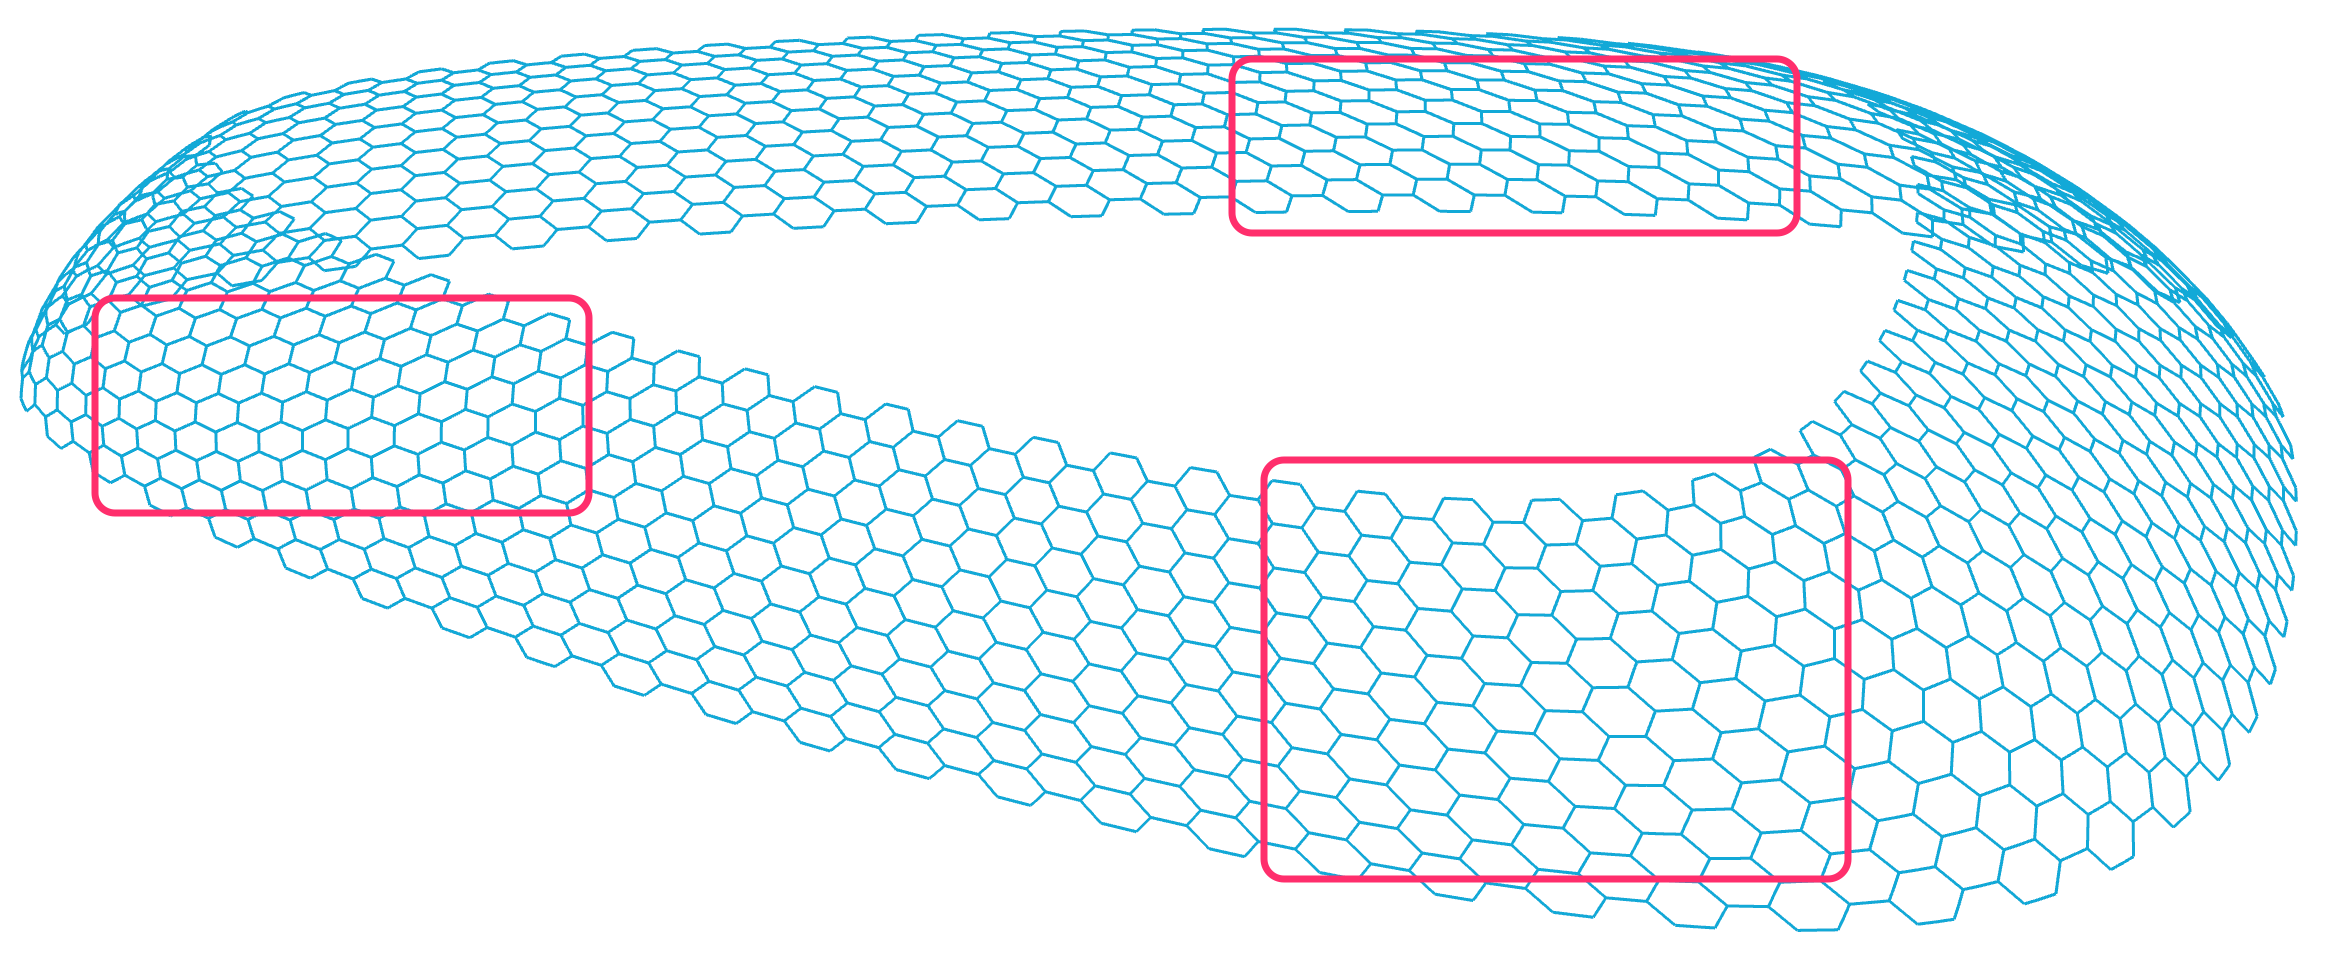
\includegraphics[width=0.32\textwidth]{images/failior-uv-marked.png}
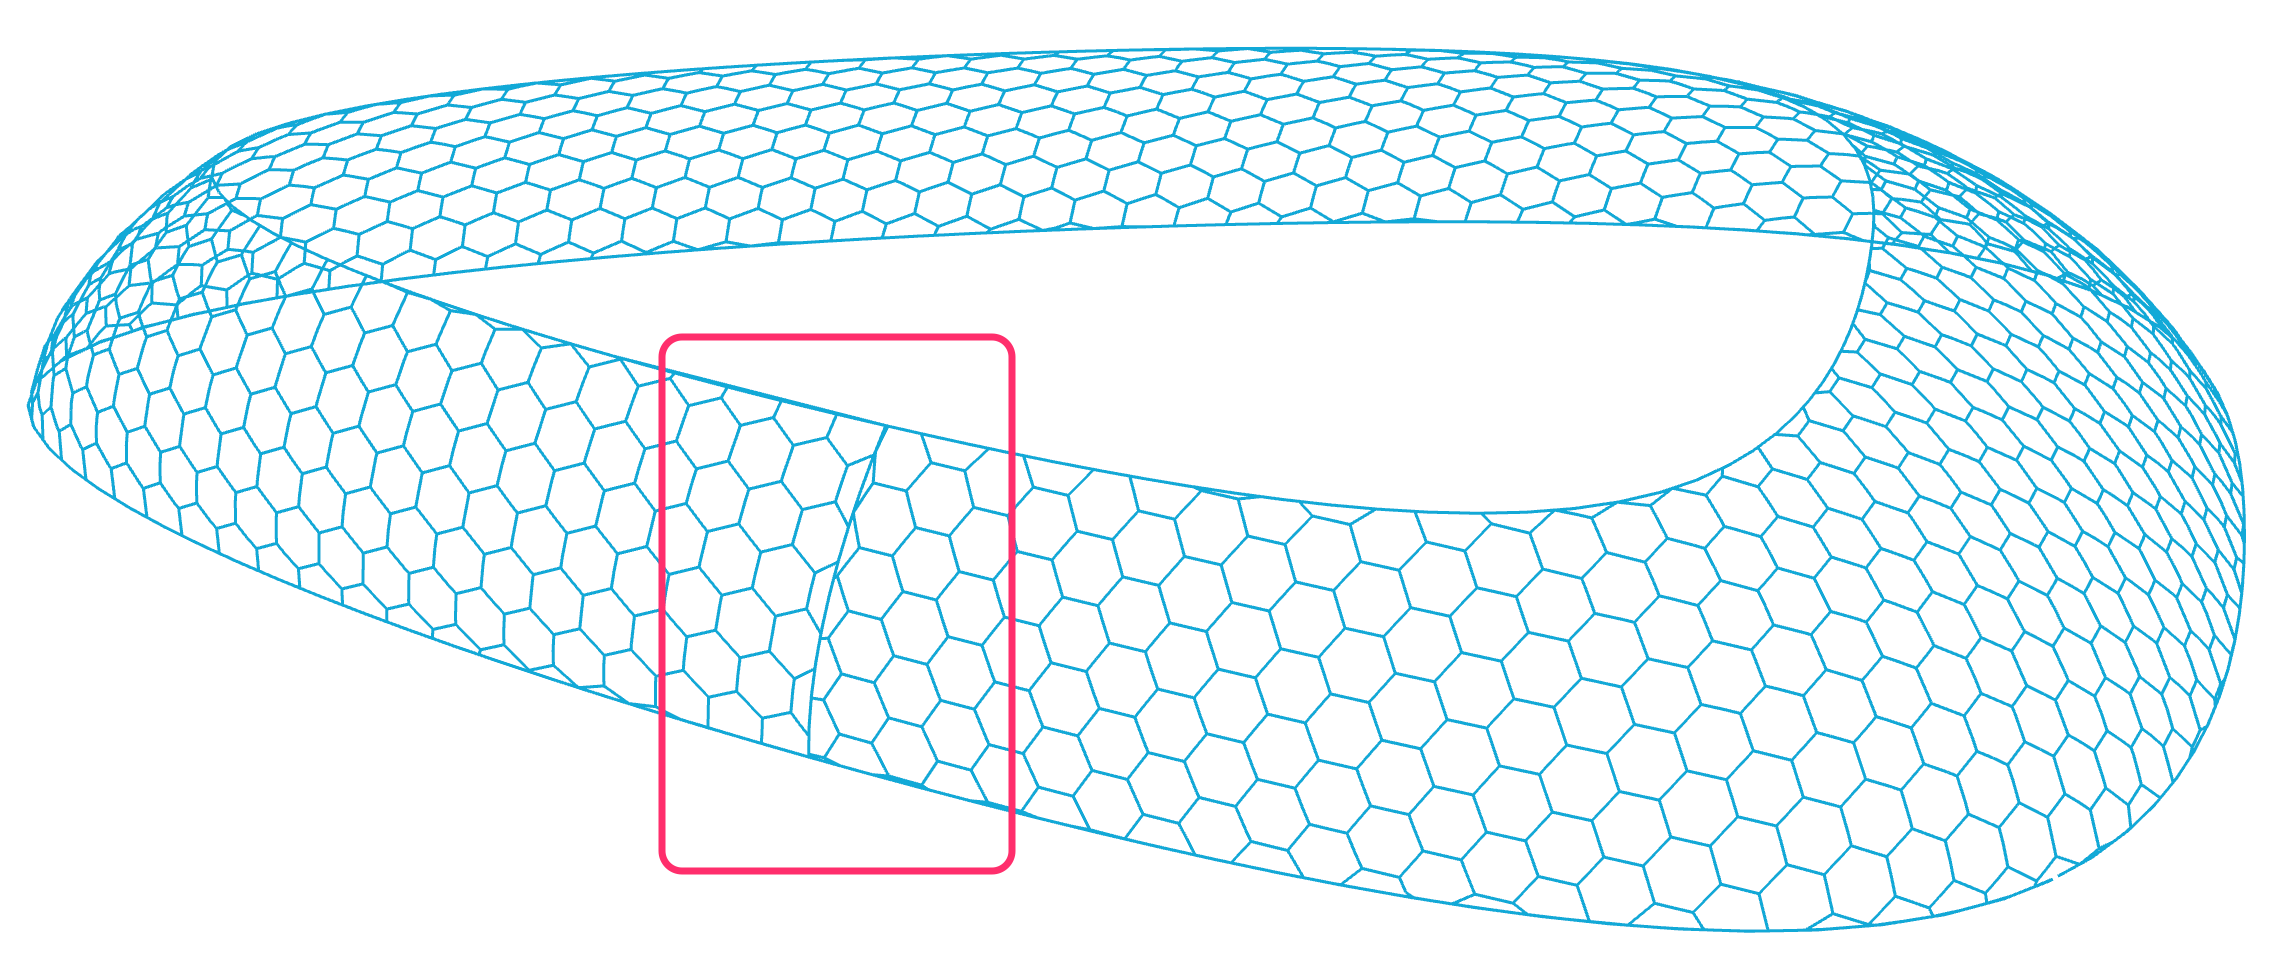
\includegraphics[width=0.32\textwidth]{images/failior-squish-marked.png}
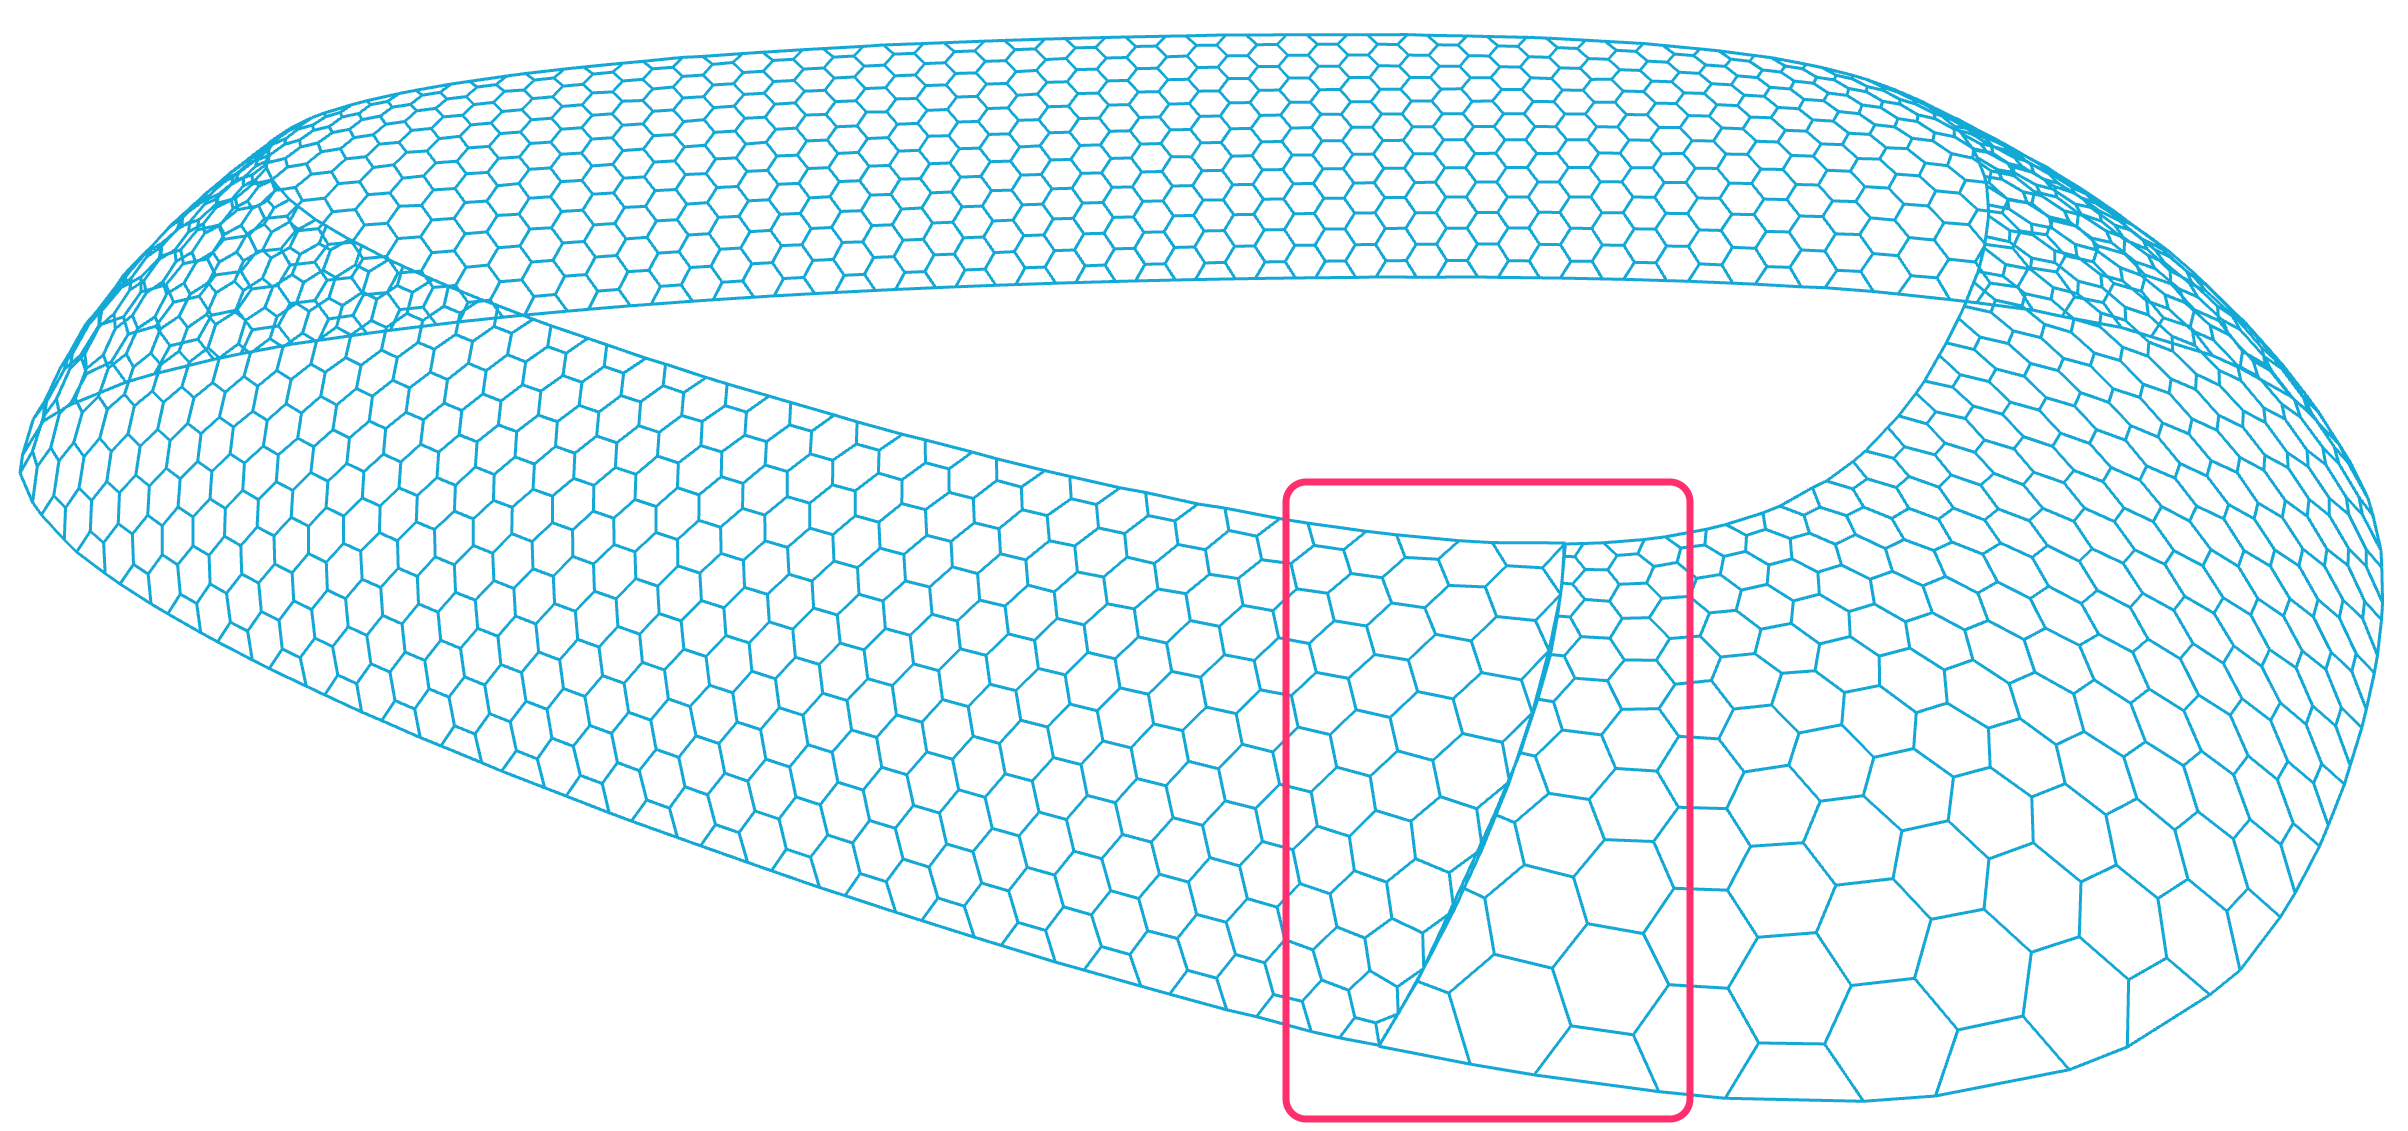
\includegraphics[width=0.32\textwidth]{images/failior-rectangle-marked.png}
\caption{State of the art unroll methods can create patterns on a closed surface.
The {\tt ApplyCrv} command of Rhinoceros produces boundary alinged periodic patterns but introduces unacceptable non-isotropic stretch (left). The {\tt SquishBack} method creates
sufficiently regular elements but does not respect the periodicity of the surface (middle).
Non-periodic conformal maps align with the boundary of a cut surface. Along the cut the 
map is not continuous (right).}
\label{fig:failure}
\end{figure}

% We illustrate different methods by describing the corresponding Rhinoceros commands
% or concepts here. 

\subsubsection{Rhinoceros CreateUVCrv/ApplyCrv.}
A \nurbs surface is naturally equipped with a parameterization, i.e.,
a UV mapping from a rectangle domain to the surface. For the surface
of Figure~\ref{fig:teaser} such a map can be used to project a pattern
from this rectangle to the surface ({\tt ApplyCrv} in Rhinoceros). The
pattern can be constructed periodically as it is defined in the UV
domain of the surface. However, in general this method does not
produce satisfactory results in terms of quality of elements for
complex freeform surfaces. The UV parameterization is not conformal
and thus introduces non-isotropic stretch and shear preventing the
elements to be regular on the surface, see Figure~\ref{fig:failure},
left. This limitation exists even for developable surfaces.

\subsubsection{Rhinoceros Squish/SquishBack.}
The {\tt Squish/SquishBack} command of Rhino maps a surface to the
plane minimizing the amount of stretch. While this is geometrically
not a conformal map it produces acceptable patterns on the surface. It
is however not capable of calculating periodic maps to the surface.
Thus it is not applicable in our situation, see
Figure~\ref{fig:failure}, middle.

\subsubsection{PanelingTools for Rhino.}
The paneling tools of Rhinoceros use the UV parameterization of the
underlying surface to populate grid-points over the surface. With the
help of such a grid, panels are placed onto the surface,
see~\cite{panelingtools}. The shapes of the panels depend heavily on
the \nurbs-parameterization. An example is shown in
Figure~\ref{fig:failure}, left.

\subsubsection{Hexagonal tilings.}
In the architectural context, hexagonal panelizations have been
studied by~\cite{TangentPlanes, Troche} and \cite{SHWP09}. These
aproaches however do not include regularity or special boundary
alignment as introduced in the current work.  In \cite{SHWP09} the
result of the panelization depends on the choice of an initial
triangle mesh that is optimized towards touching incircles. This
allows for a torsion free support structure of a non planar
hex-mesh. Hexagonal tilings for triangulated surfaces also have been
studied by \cite{NieserPPZ12}. They focus on regularity but not on
boundary conditions.

\subsubsection{Mesh parameterizations.}
There are a vast number of parameterization schemes for meshes. To
elaborate on all methods is beyond the scope of this section and we
describe only the most relevant results here. General purpose
parameterization methods for triangle meshes produce high quality quad
or hex meshes for unstructured input data, see for
instance~\cite{Bommes2009, ARAP, SSP08}. They have been used with
success in the architectural context, e.g., by~\cite{bo-2011-cas} and
\cite{SRB12}.

The basis of our method are conformally equivalent triangle meshes as
described by \cite{SSP08}. The straight forward method to map a
surface with this approach is to cut it open and map it to a rectangle
domain. This method yields boundary aligned conformal maps that
however do not match along the introduced cut, see
Figure~\ref{fig:failure}, right. How to generalize this method to
overcome this limitation is the content of the following section.

\subfilebibliography

\end{document}

%%% Local Variables: 
%%% mode: latex
%%% TeX-master: "article"
%%% End: 
